\section{数值实验与结果}
\label{sec:experiments}

本节给出若干数值算例，用于系统评估 DeepRTE 在辐射传输方程求解中的精度与效率。实际应用中，RTE~\eqref{eq:rte} 定义在三维空间变量 $\br\in\mathbb{R}^3$ 与角变量 $\bOmega\in\sS^2$ 上，对应 $d=3$，因此为六维问题。通过适当的变量变换与对称性分析，可以将其约化为低维模型，从而降低数值计算的整体复杂度。

在笛卡尔坐标系下，记
\begin{equation}
    \bOmega=(c,s,\zeta), \quad c =
        {\left(1-\zeta^{2}\right)}^{\frac{1}{2}} \cos\theta, \quad s =
        {\left(1-\zeta^{2}\right)}^{\frac{1}{2}} \sin\theta, \quad \text{for }|\zeta| \leq 1.
\end{equation}
令总截面 $\mut$ 与散射截面 $\mus$ 仅依赖于平面坐标 $(x,y)$，且强度 $I$ 在 $z$ 方向上均匀，则定义
\begin{equation}
    \tilde{I}(x, y,\zeta,\theta) = \frac{1}{2}\bigl[I(x,y,z,c,s,\zeta) + I(x,y,z,c,s,-\zeta)\bigr],
\end{equation}
以及
\begin{equation}
    \tilde{p}(\zeta,\theta,\zeta^*, \theta^*) = \frac{1}{2}\bigl[p(c,s,\zeta, c^*,s^*,\zeta^*) + p(c,s,\zeta, c^*,s^*,-\zeta^*)\bigr],
\end{equation}
则两者均与 $z$ 无关，且关于 $\zeta$ 为偶函数。由此，方程~\eqref{eq:rte-with-bc} 可约化为
\begin{equation}
    \bigl(c\partial_x \tilde{I}(x,y,\zeta,\theta)+s\partial_y
    \tilde{I}(x,y,\zeta,\theta)\bigr)+\mut \,\tilde{I}(x,y,\zeta,\theta)=\frac{\mus}{2\pi}\int_{0}^{1}
    \int_0^{2\pi} \tilde{p}(\zeta, \theta, \zeta^*,\theta^*) \,\tilde{I}(x,y,\zeta^*,\theta^*) \,\diff{\theta^*}\diff{\zeta^*},
\end{equation}
配以入射边界条件
\begin{equation}
    \tilde{I}(x,y,\bOmega)=\tilde{I}_{-}(x,y,\bOmega), \quad \text{当 }
    \bOmega\cdot\bm{n}<0,\quad (x, y)\in\partial D.
\end{equation}

相函数 $p$ 是辐射传输方程中的关键组成部分，通常仅依赖入射与出射方向之间的夹角。本文采用归一化的 Henyey--Greenstein（H-G）相函数作为各向异性散射的代表性模型：
\begin{equation}
    p(\bOmega,\bOmega^*) = p(\bOmega\cdot\bOmega^*) = \frac{1-g^2}{{\Bigl(1+g^2-2g\,(cc^*+ss^*+\zeta\zeta^*)\Bigr)}^{\frac{3}{2}}}.
\end{equation}
其中参数 $g$ 控制前向与后向散射的相对权重：$g=0$ 时对应各向同性散射，$g\to 1$ 时则对应高度前向集中的散射。虽然本文数值实验均基于 H-G 相函数，但算法本身可直接推广到其他散射模型。

\subsection{数据集构造}\label{sec:dataset-construction}

训练集与测试集均由传统数值方法生成，主要采用扫掠法（sweeping method）。
\todo[inline]{~\cite{koch1991solution,zeyao2004parallel}}
相应的 MATLAB 与 Python 实现已开源于 \href{https://github.com/mazhengcn/rte-dataset}{rte-dataset} 仓库，便于复现实验与进行进一步比较。

\paragraph{计算区域与离散}
数值实验在矩形空间区域 $D = [0, 1]\times[0, 1]\subset \mathbb{R}^2$ 以及角度空间 $\mathbb{S}^{2}$ 上进行。每个空间方向均采用 $40$ 个等间距网格点。

\paragraph{角度求积点}
角度求积点选取为区间 $[-1,1]$ 上 $2N$ 阶标准勒让德多项式的正根。本文取 $N=3$，对应的求积点与权重列于表~\ref{tab:quadrature}。

\begin{table}[!htp]
    \centering
    \begin{tabular}{ccccc}
        \toprule
        $\zeta_i$ & $\theta_i$ & $c_i$     & $s_i$     & $4 w_i$   \\
        \midrule
        0.2386192 & $\pi$/12   & 0.9380233 & 0.2513426 & 0.1559713 \\
        0.2386192 & 3$\pi$/12  & 0.6866807 & 0.6866807 & 0.1559713 \\
        0.2386192 & 5$\pi$/12  & 0.2513426 & 0.9380233 & 0.1559713 \\
        0.6612094 & $\pi$/8    & 0.6930957 & 0.2870896 & 0.1803808 \\
        0.6612094 & 3$\pi$/8   & 0.2870896 & 0.6930957 & 0.1803808 \\
        0.9324695 & $\pi$/4    & 0.2554414 & 0.2554414 & 0.1713245 \\
        \bottomrule
    \end{tabular}
    \bicaption{角度求积点及其权重。$\zeta_i$ 与 $\theta_i$ 为速度空间求积点，$c_i$ 与 $s_i$ 分别为对应的余弦与正弦值，$w_i$ 为求积权重。}{Angular quadrature points and weights of the quadrature set. $\zeta_i$ and $\theta_i$ are the quadrature points of the velocity space, $c_i$ and $s_i$ are the corresponding cosine and sine values, and $w_i$ is the quadrature weight.}\label{tab:quadrature}
\end{table}

\paragraph{截面系数}
总截面 $\mu_t(x,y)$ 与散射截面 $\mu_s(x,y)$ 在子区域 $D_\mu = [0.4, 0.6] \times [0.4, 0.6]$ 上随机取值，其余区域取常数，具体定义为
\begin{equation} \label{eq:coefficients_definition}
    \begin{aligned}
        \mu_t(x,y) & =
        \begin{cases}
            U_t, \quad \text{其中 } U_t \sim \mathcal{U}(5,7), & \text{若 } (x,y) \in D_\mu,    \\
            10,                                              & \text{若 } (x,y) \notin D_\mu,
        \end{cases} \\
        \mu_s(x,y) & =
        \begin{cases}
            U_s, \quad \text{其中 } U_s \sim \mathcal{U}(2,4), & \text{若 } (x,y) \in D_\mu,    \\
            5,                                               & \text{若 } (x,y) \notin D_\mu.
        \end{cases}
    \end{aligned}
\end{equation}

\paragraph{训练集边界条件}
训练数据集中采用 Delta 函数型入射边界条件，并用高斯函数进行近似。入射边界条件具体为
\begin{equation}\label{eq:bc-condition}
    \centering
    \left \{ % tex-fmt: skip
    \begin{aligned}
         & I_-(x=0,y,c>0,s;x_l^{\prime}=0,
        y_l^{\prime},c_l^{\prime},s_l^{\prime})
        =\delta_{\{y_l^{\prime}\}}^{\sigma_{\br}}(y)\delta^{\sigma_{\bOmega}}(c - c_l')\delta^{\sigma_{\bOmega}}(s - s_l'),
        \\
         & I_-(x=1,y,c<0,s;x_r^{\prime}=1,
        y_r^{\prime},c_r^{\prime},s_r^{\prime})
        =\delta_{\{y_r^{\prime}\}}^{\sigma_{\br}}(y)\delta^{\sigma_{\bOmega}}(c - c_r')\delta^{\sigma_{\bOmega}}(s - s_r'),
        \\
         & I_-(x,y=0,c,s>0;x_b^{\prime},y_b^{\prime}=0, c_b^{\prime},
        s_b^{\prime})
        =\delta_{\{x_b^{\prime}\}}^{\sigma_{\br}}(x)\delta^{\sigma_{\bOmega}}(c - c_b')\delta^{\sigma_{\bOmega}}(s - s_b'),
        \\
         & I_-(x,y=1,c,s<0;x_t^{\prime},y_t^{\prime}=1,c_t^{\prime},
        s_t^{\prime})
        =\delta_{\{x_t^{\prime}\}}^{\sigma_{\br}}(x)\delta^{\sigma_{\bOmega}}(c - c_t')\delta^{\sigma_{\bOmega}}(s - s_t'),
    \end{aligned}
    \right. % tex-fmt: skip
\end{equation}
其中，$y_l'$（left）、$y_r'$（right）、$x_b'$（bottom）与 $x_t'$（top）分别为对应边界上高斯束中心的坐标，从离散网格点中均匀随机选取。角变量 $c_l'$、$c_r'$、$c_b'$、$c_t'$ 及 $s_l'$、$s_r'$、$s_b'$、$s_t'$ 则从满足入射条件的离散速度方向中均匀采样。空间与角度方向上的尺度参数分别满足
\begin{equation}
    \sigma_{\br} \sim \mathcal{U}(0.005\sqrt{2},0.02\sqrt{2}), \quad \sigma_{\bOmega} \sim \mathcal{U}(0.005\sqrt{2},0.01\sqrt{2}).
\end{equation}

\paragraph{数据归一化}
在训练过程中，将强度 $I$ 归一化到区间 $[0, 1]$：
\begin{equation}
    I_{\text{norm}} = \frac{I - I_{\text{min}}}{I_{\text{max}} - I_{\text{min}}},
\end{equation}
其中 $I_{\text{min}}$ 与 $I_{\text{max}}$ 分别为数据集中观测到的最小与最大强度值。该归一化有助于稳定训练过程并提升收敛性能。

\paragraph{散射参数区间}
模型在三种不同散射强度区间上进行训练与测试，这些区间由散射不对称参数 $g\in[0,1]$ 划分：$g=0$ 表示各向同性散射，$g=1$ 表示极端前向散射。具体区间为
\begin{itemize}
    \item \textbf{近各向同性（Near isotropy）}: $ g \sim \mathcal{U}(0, 0.2)$，对应几乎各向同性散射，即粒子在各方向散射概率接近相同；
    \item \textbf{中度各向异性（Moderate anisotropy）}: $ g \sim \mathcal{U}(0.4, 0.6)$，对应中等强度的各向异性散射；
    \item \textbf{强前向散射（Highly forward peaking）}: $ g \sim \mathcal{U}(0.7, 0.9)$，对应粒子主要沿前向传播的强各向异性情形，此时粒子轨迹高度相关、位置与散射方向紧密耦合，边界条件的微小变化也可能显著影响解的行为。
\end{itemize}

上述数据集构造所用的超参数汇总于表~\ref{tab:dataset}。
\begin{table}[!htp]
    \centering
    \begin{tabular}{lp{0.3\textwidth}ll}
        \toprule
        类别                                         & 参数                                            & 符号                       & 取值/范围                                \\ \midrule
        \multirow{2}{*}{空间区域（Spatial domain）}      & 计算区域（Domain）                                  & $D$                      & ${[0,1]}^2$                          \\
                                                   & 子区域（Subdomain）                                & $D_\mu$                  & ${[0.4,0.6]}^2$                      \\
        \midrule
        \multirow{4}{*}{截面系数（Cross section）}       & \multirow{2}{*}{总截面（Total）}                   & \multirow{2}{*}{$\mut$}  & $D_\mu$ 内：$\mathcal{U}(5,7)$         \\
                                                   &                                               &                          & $D\backslash D_\mu$ 内：$10$           \\
                                                   & \multirow{2}{*}{散射截面（Scattering）}             & \multirow{2}{*}{$\mus$}  & $D_\mu$ 内：$\mathcal{U}(2,4)$         \\
                                                   &                                               &                          & $D\backslash D_\mu$ 内：$5$            \\
        \midrule
        \multirow{2}{*}{离散化（Discretization）}       & 空间网格点数（\# of mesh points）                     & $N_{\text{mesh}}$        & 40                                   \\
                                                   & 角度求积点数（\# of angular quadrature points）       & $N_\text{quad}$          & 24                                   \\ \midrule
        \multirow{5}{*}{边界条件（Boundary conditions）} & 光束空间中心坐标（Beam spatial centers）                & $y_l', y_r', x_b', x_t'$ & 从网格点中随机采样                            \\
                                                   & \multirow{2}{*}{光束角度求积点（Beam angular points）} & $c_l', c_r', c_b', c_t'$ & \multirow{2}{*}{从角度求积点中随机采样}         \\
                                                   &                                               & $s_l', s_r', s_b', s_t'$ &                                      \\
                                                   & 光束空间标准差（Beam spatial std dev）                 & $\sigma_{\br}$           & $\sqrt{2}\,\mathcal{U}(0.005, 0.02)$ \\
                                                   & 光束角度标准差（Beam angular std dev）                 & $\sigma_{\bOmega}$       & $\sqrt{2}\,\mathcal{U}(0.005, 0.01)$ \\
        \midrule
        \multirow{3}{*}{散射参数（Scattering）}          & \multirow{3}{*}{不对称参数（Asymmetry parameter）}   & \multirow{3}{*}{$g$}     & $\mathcal{U}(0,0.2)$                 \\
                                                   &                                               &                          & $\mathcal{U}(0.4,0.6)$               \\
                                                   &                                               &                          & $\mathcal{U}(0.7,0.9)$               \\
        \bottomrule
    \end{tabular}
    \bicaption{数据集构造中使用的超参数汇总。表中给出了计算区域、截面系数、离散参数、边界条件以及散射参数等设置。}{Summary of hyperparameters for dataset construction. This table details the computational domain, cross sections, discretization, boundary conditions, and other parameters used.}\label{tab:dataset}
\end{table}

\subsection{训练细节}

\paragraph{训练配置}

\begin{table}[!htp]
    \centering
    \begin{tabular}{ll}
        \toprule
        超参数（Hyperparameters）  & 取值（Value）                  \\ \midrule
        优化器（Optimizer）        & Adam                       \\
        学习率策略（Schedule）       & 余弦退火（Cosine annealing）     \\
        初始学习率                 & $1 \times 10^{-3}$         \\
        批大小（Batch size）       & 8                          \\
        训练轮数（Epochs）          & 5000                       \\
        训练样本数                 & 800                        \\
        验证样本数                 & 200                        \\
        配点数量（Collocation pts） & 128                        \\
        硬件（Hardware）          & 4$\times$ NVIDIA 4090 GPUs \\
        \bottomrule
    \end{tabular}
    \bicaption{模型训练超参数汇总。表中列出了优化器、学习率策略与初值、数据规模以及硬件配置等信息。}{Summary of model training hyperparameters. This table details the optimizer and training hyperparameters, including learning rate, dataset settings, and hardware information.}
    \label{tab:training_details}
\end{table}

模型训练采用 Adam 优化器与余弦退火（cosine annealing）学习率策略。对每个散射区间，各生成 $800$ 个训练样本与 $200$ 个验证样本。训练在四张 NVIDIA RTX 4090 GPU 上进行，共训练 $5000$ 个 epoch。初始学习率设为 $1 \times 10^{-3}$，batch size 取 $8$，损失函数中使用的 collocation 点数（见~\eqref{eq:collocation_points}）为 $128$。训练超参数如表~\ref{tab:training_details} 所示。

\paragraph{网络结构}
DeepRTE 的网络超参数列于表~\ref{tab:parameters}。网络由衰减模块与散射模块两部分构成，对应的层数、隐含维度、输出维度、多头注意力头数以及潜在特征维度等均在表中给出。

\begin{table}[!htp]
    \centering
    \begin{tabular}{lll}
        \toprule
        Module Name                  & Hyperparameters                          & Value \\ \midrule
        \multirow{7}{*}{Attenuation} & \texttt{num\_layer}
        $N_{\text{mlp}}$             & 4                                                \\
                                     & \texttt{hidden\_dim}  $d_{\text{mlp}}$   & $128$ \\
                                     & \texttt{output\_dim}  $d_{\text{model}}$ & $16$  \\
                                     & \texttt{num\_head}    $N_{\text{head}}$  & $2$   \\
                                     & \texttt{key\_dim}     $d_k$              & $32$  \\
                                     & \texttt{value\_dim}   $d_v$              & $32$  \\
                                     & \texttt{output\_dim}  $d_{\tau}$         & $2$   \\
        \midrule
        \multirow{2}{*}{Scattering}  & \texttt{num\_block}   $N_{\ell}$         & $2$   \\
                                     & \texttt{latent\_dim}  $d_{\text{model}}$ & $16$  \\
        \bottomrule
    \end{tabular}
    \bicaption{DeepRTE 网络超参数。网络由衰减模块与散射模块两部分构成，表中给出了层数、隐含维度、输出维度、多头数、键/值维度以及潜在特征维度等。}{DeepRTE network hyperparameters. The network consists of two modules: the attenuation module and the scattering module. The hyperparameters include the number of layers, hidden dimensions, output dimensions, number of heads, key dimensions, value dimensions, and latent dimensions.}\label{tab:parameters}
\end{table}

\subsection{结果分析}
\subsubsection{精度验证}
\label{sec:acc}

本小节评估 DeepRTE 的数值精度与计算效率。精度指标采用预测结果与真值之间的均方误差（MSE）以及均方根百分比误差（RMSPE）。所有结果均基于与训练集分布一致的验证数据集。

\begin{table}[!htp]
    \centering
    \begin{tabular}{@{}cccccc@{}}
        \toprule
        模型（Model）                & 参数量（\# of parameters）  & 散射区间（Scattering regime）       & $g$ 取值范围   & MSE ($\times 10^{-10}$) & RMSPE (\%) \\ \midrule
        \multirow{3}{*}{DeepRTE} & \multirow{3}{*}{37954} & 近各向同性（Near isotropy）          & (0, 0.2)   & 5.630                   & 2.827      \\ \cmidrule(l){3-6}
                                 &                        & 中度各向异性（Moderate anisotropy）   & (0.4, 0.6) & 5.453                   & 2.759      \\ \cmidrule(l){3-6}
                                 &                        & 强前向散射（Highly forward peaking） & (0.7, 0.9) & 7.223                   & 3.181      \\ \bottomrule
    \end{tabular}
    \bicaption{DeepRTE 在三种散射区间上的精度指标。所有验证样本与训练集分布一致，表中给出了各区间上的 MSE 与 RMSPE，均表现出较高精度。}{Accuracy validation of DeepRTE model across three distinct scattering regimes. All validation experiments were conducted on a dataset sharing the same distribution as the training dataset. The table demonstrates that the model achieves high accuracy with RMSPE consistently below 3.2\% across all regimes.}\label{tab:accuracy}
\end{table}

从表~\ref{tab:accuracy} 可见，在所有散射区间内，DeepRTE 的 MSE 均不超过 $7.3 \times 10^{-10}$，RMSPE 控制在 $3.2\%$ 以内，表明模型在不同散射强度下均具有较高精度。具体而言，在近各向同性区间中，MSE 为 $5.630 \times 10^{-10}$，RMSPE 为 $2.827\%$，在几乎各向同性情形下表现优异；在中度各向异性区间中，MSE 略有降低（$5.453 \times 10^{-10}$），RMSPE 为 $2.759\%$，精度相当；在强前向散射区间中，由于散射高度各向异性，问题更具挑战性，但模型仍能保持 $7.223 \times 10^{-10}$ 的 MSE 与 $3.181\%$ 的 RMSPE，反映出良好的鲁棒性。

表~\ref{tab:accuracy-figs} 给出了三个散射区间中代表性算例的可视化对比结果。对每个区间，我们依次展示：密度 $\Phi$ 的三维真值、二维投影真值、模型预测以及二者之差的绝对误差。

表~\ref{tab:time_compare} 给出了 DeepRTE 与传统方法在运行时间上的对比，用以体现本方法在效率方面的优势。快速扫掠法分别采用 CPU 与 GPU 两种实现：CPU 版本基于 Python（NumPy 与 SciPy），在 Intel(R) Xeon(R) Silver 4410Y（12 核）上运行，耗时约 $193.0$ 秒；GPU 版本基于 JAX，在多个设备之间进行数据分片、采用多 GPU 并行与 \texttt{jax.jit} JIT 编译（见算法~\ref{alg:fast-sweeping-gpu}），在 $4\times$ NVIDIA GeForce RTX 4090 上耗时约 $16.7$ 秒，相比 CPU 提升约 $11.6$ 倍。相比之下，DeepRTE 在相同的 $4\times$ RTX 4090 上完成一次推理仅需 $2.3$ 秒，相比 GPU 快速扫掠法进一步加速约 $7.3$ 倍，相比 CPU 基线则加速约 $83.9$ 倍，推理效率优势十分显著。

这些结果表明，DeepRTE 在不同散射参数设置下均能够较好地捕捉散射物理过程，在复杂的前向散射场景中仍能保持较低误差；同时，模型参数量仅约 $3.8\times 10^4$，推理效率较高，适合大规模高效模拟场景。

\begin{table}[!htp]
    \centering
    \begin{tabular}{@{}lccc@{}}
        \toprule
        方法（Method）   & 设备（Device）                    & 计算单元数量（Count） & 时间 Time (s) \\ \midrule
        快速扫掠法（CPU）   & Intel(R) Xeon(R) Silver 4410Y & 12 核（cores）   & 193.0       \\
        快速扫掠法（GPU）   & NVIDIA GeForce RTX 4090       & 4 GPUs        & 16.7        \\
        \midrule
        DeepRTE（GPU） & NVIDIA GeForce RTX 4090       & 4 GPUs        & 2.3         \\ \bottomrule
    \end{tabular}
    \bicaption{不同方法在 CPU 与 GPU 上的运行时间对比。快速扫掠法在 CPU 与 GPU 上分别耗时 193.0 s 与 16.7 s，而 DeepRTE 在 $4\times$ RTX 4090 上仅需 2.3 s，显著提升了推理效率。}{Runtime comparison. The conventional fast sweeping method requires 193.0 s on an Intel(R) Xeon(R) Silver 4410Y (12 cores) and 16.7 s on $4\times$ NVIDIA GeForce RTX 4090 GPUs ($11.6\times$ over CPU). By contrast, DeepRTE completes inference in 2.3 s on $4\times$ RTX 4090, achieving a $7.3\times$ speedup over the GPU fast sweeping method and an $83.9\times$ speedup relative to the CPU baseline.}
    \label{tab:time_compare}
\end{table}

\begin{algorithm}[!htp]
    \caption{多 GPU 快速扫掠法（Multi-GPU Fast-Sweeping Method）}\label{alg:fast-sweeping-gpu}
    \SetAlgoLined
    \KwIn{$\mut, \mus, \{c_k\}, \{s_k\}, \{w_{k'}\}, p, \Delta x, \Delta y, D, \text{tol}, \text{max\_iter}$}
    \KwOut{$I$}

    \BlankLine

    \emph{在 $D$ 个设备之间划分角通量与散射核}
    $M \gets n_v / D$\;

    \For{$d = 1,\dots,D$}{%
    \emph{在第 $d$ 个设备上初始化角通量与散射核，并复制截面系数}\
    $I^{d,[\ell]}_{i,j,k} \gets 0,\quad I^{d,[\ell]}_{i,j,k} \in \mathbb{R}^{n_x \times n_y \times M}$\;
    $p^d_{k,k'} \gets p_{k,k'},\quad k \in [(d-1)M, dM),\; k' \in [0,n_v)$\;
    $\mu_t^d,\mu_s^d \gets \mu_t,\mu_s$\;
    }

    \BlankLine

    \For{$\ell = 0,1,\dots,\text{max\_iter}-1$}{%
    \emph{步骤 1：跨设备收集角通量（全收集通信）}\
    $I^{[\ell]}_{i,j,k'} \gets \text{All-Gather}(\{I^{d,[\ell]}_{i,j,k}\}_{d=1}^D),\quad k' \in [0,n_v)$\;

    \emph{步骤 2：在各设备上计算局部散射矩（本地计算，无通信）}\
    \For{$d = 1,\dots,D$}{%
    $S^{d,[\ell]}_{i,j,k} \gets \displaystyle\sum_{k'=0}^{n_v-1} w_{k'}\,p^d_{k,k'}\,I^{[\ell]}_{i,j,k'},\quad k \in [(d-1)M, dM)$\;
    }

    \emph{步骤 3：在各设备上执行角度扫掠（本地计算，无通信）}\
    \For{$d = 1,\dots,D$}{%
    \For{$(i,j)$ \text{ in sweep order}}{%
    $I^{d,[\ell+1]}_{i,j,k} \gets \dfrac{c_k\dfrac{I^{d,[\ell]}_{i-1,j,k}}{\Delta x} + s_k\dfrac{I^{d,[\ell]}_{i,j-1,k}}{\Delta y} + (\mu_s)_{i,j}\,S^{d,[\ell]}_{i,j,k}}{\dfrac{c_k}{\Delta x} + \dfrac{s_k}{\Delta y} + (\mu_t)_{i,j}},\quad k \in [(d-1)M, dM)$\;
    }
    }

    \emph{步骤 4：检查收敛性}\
    \If{$\text{RelativeError}(I^{[\ell+1]}, I^{[\ell]}) < \text{tol}$}{%
        extbf{break}\;
    }
    }

    \BlankLine

    \emph{在所有设备之间收集最终角通量}\
    $I^{[\ell]} \gets \text{All-Gather}(\{I^{d,[\ell]}\}_{d=1}^D)$\;

    \Return{$I^{[\ell]}$}\;
\end{algorithm}

\begin{table}[!htp]
    \centering
    \begin{tabular}{>{\centering\arraybackslash}m{0.9cm}cccc}
        \toprule
        $g$                         & $\Phi_{\text{label}}$                                             & $\Phi_{\text{label}}$                                          & $\Phi_{\text{predict}}$                                      & $|\Phi_{\text{label}}- \Phi_{\text{predict}}|$                 \\
        \midrule
        \raisebox{5em}{$(0,0.2)$}   & 
\includegraphics[width=0.22\textwidth]{val_g0.1_phi_label_3d.pdf} & 
\includegraphics[width=0.20\textwidth]{val_g0.1_phi_label.pdf} & 
\includegraphics[width=0.20\textwidth]{val_g0.1_phi_pre.pdf} & 
\includegraphics[width=0.20\textwidth]{val_g0.1_phi_error.pdf} \\
        \raisebox{5em}{$(0.4,0.6)$} & 
\includegraphics[width=0.22\textwidth]{val_g0.5_phi_label_3d.pdf} & 
\includegraphics[width=0.20\textwidth]{val_g0.5_phi_label.pdf} & 
\includegraphics[width=0.20\textwidth]{val_g0.5_phi_pre.pdf} & 
\includegraphics[width=0.20\textwidth]{val_g0.5_phi_error.pdf} \\
        \raisebox{5em}{$(0.7,0.9)$} & 
\includegraphics[width=0.22\textwidth]{val_g0.8_phi_label_3d.pdf} & 
\includegraphics[width=0.20\textwidth]{val_g0.8_phi_label.pdf} & 
\includegraphics[width=0.20\textwidth]{val_g0.8_phi_pre.pdf} & 
\includegraphics[width=0.20\textwidth]{val_g0.8_phi_error.pdf} \\
        \bottomrule
    \end{tabular}
    \bicaption{不同散射区间下密度 $\Phi$ 预测结果的可视化比较：包括三维与二维真值、模型预测以及绝对误差图。}{Visual comparison of density $\Phi$ predictions across scattering regimes: ground truth (3D and 2D views), model predictions, and absolute errors for representative validation cases.}\label{tab:accuracy-figs}
\end{table}

\begin{figure}[!htp]
    \centering
    
\includegraphics[width=\textwidth]{train_loss.pdf}
    \bicaption{在 Delta 函数训练数据集上训练所得的损失曲线，展示了随 epoch 推进的收敛行为。}{Loss curve. Obtained from training the model on a delta function training dataset, illustrating the convergence behavior over epochs.}\label{fig:loss}
\end{figure}

\subsubsection{线性性质验证}\label{sec:linearity_val}

DeepRTE 的网络结构在设计时就有意保持了对入射边界函数 $I_{-}$ 的线性性质。根据~\eqref{eq:greens-integral-nn}，DeepRTE 中使用的神经网络 $G^{\text{NN}}$ 以积分形式表征了解算子 $\ANN$ 的核（即格林函数），因此在连续和离散层面上，DeepRTE 从 $I_{-}$ 到解的整体映射应当保持线性。

为验证这一结论，本节通过数值实验证明模型同时满足可加性与齐次性两条基本线性性质。所有实验均在固定的截面系数 $\mu_t,\mu_s$ 与相函数 $p$ 条件下进行，其具体设置为
\begin{equation}
    \mu_t(x,y) =
    \begin{cases}
        6,  & \text{若 } (x,y) \in D_\mu,    \\
        10, & \text{若 } (x,y) \notin D_\mu,
    \end{cases}
    \quad
    \mu_s(x,y) =
    \begin{cases}
        3, & \text{若 } (x,y) \in D_\mu,    \\
        5, & \text{若 } (x,y) \notin D_\mu,
    \end{cases}
    \quad
    g=0.5, \quad D_\mu = [0.4, 0.6]^2.
\end{equation}
下文中，记 DeepRTE 解算子为 $\ANN$（省略参数依赖）。

\paragraph{1. 可加性检验}
线性可加性要求：对应于两个入射边界之和的预测解，应等于分别求解后二者解的和，即
\begin{equation}\label{eq:additivity-val}
    \ANN(I_{-}^{(1)} + I_{-}^{(2)}) = \ANN I_{-}^{(1)} + \ANN I_{-}^{(2)}.
\end{equation}
我们首先选取验证集中的两个独立入射边界条件 $I_{-}^{(1)}$ 与 $I_{-}^{(2)}$，其形式均为~\eqref{eq:bc-condition}，并取
\begin{equation}
    I_{-}^{(1)}:
    \begin{cases}
        y_l'=0.3875,\; y_r'=0.6125,\; x_b'=0.6125,\; x_t'=0.3875,   \\
        c_l'=0.6931,\; c_r'=-0.6931,\; c_b'=0.2871,\; c_t'=-0.2871, \\
        s_l'=-0.2871,\; s_r'=0.2871,\; s_b'=0.6931,\; s_t'=-0.6931,
    \end{cases}
\end{equation}
以及
\begin{equation}
    I_{-}^{(2)}:
    \begin{cases}
        y_l'=0.1375,\; y_r'=0.8625,\; x_b'=0.8625,\; x_t'=0.1375,   \\
        c_l'=0.2871,\; c_r'=-0.2871,\; c_b'=-0.6931,\; c_t'=0.6931, \\
        s_l'=0.6931,\; s_r'=-0.6931,\; s_b'=0.2871,\; s_t'=-0.2871.
    \end{cases}
\end{equation}
此处方差取 $\sigma_{\br}=0.01$、$\sigma_{\bOmega}=0.0075$。我们计算~\eqref{eq:additivity-val} 左右两侧的 MSE：
\begin{equation}
    \ell(\ANN (I_{-}^{(1)}{+}I_{-}^{(2)}),\ANN I_{-}^{(1)} + \ANN I_{-}^{(2)})=1.581\times 10^{-19},
\end{equation}
可见二者几乎完全重合，从而验证了 DeepRTE 的可加性。

进一步地，我们比较合成边界 $I_{-}^{(1)}{+}I_{-}^{(2)}$ 下 DeepRTE 预测解 $\ANN (I_{-}^{(1)}{+}I_{-}^{(2)})$ 与数值求解器所得真解 $\mathcal{A}(I_{-}^{(1)}{+}I_{-}^{(2)})$ 之间的误差：MSE 为 $1.358\times10^{-8}$，RMSPE 为 $2.83\%$，说明模型在合成边界条件下仍能保持较高精度。相应的密度 $\Phi$ 可视化结果见图~\ref{fig:additivity}。

为了更一般地验证可加性，我们还在 100 个验证样本上进行统计实验。对每个样本的边界条件 $I_{-}^{(1)}$，随机选取另一样本边界 $I_{-}^{(2)}$，构造合成边界 $I_{-}^{(1)}{+}I_{-}^{(2)}$，并比较~\eqref{eq:additivity-val} 两侧。此时 MSE 与 RMSPE 分别为 $1.421\times 10^{-19}$ 与 $9.20\times10^{-6}\%$（见表~\ref{tab:linearity}），进一步印证了可加性。

\begin{figure}[!htp]
    \centering
    \begin{subfigure}[b]{0.30\textwidth}
        \centering
        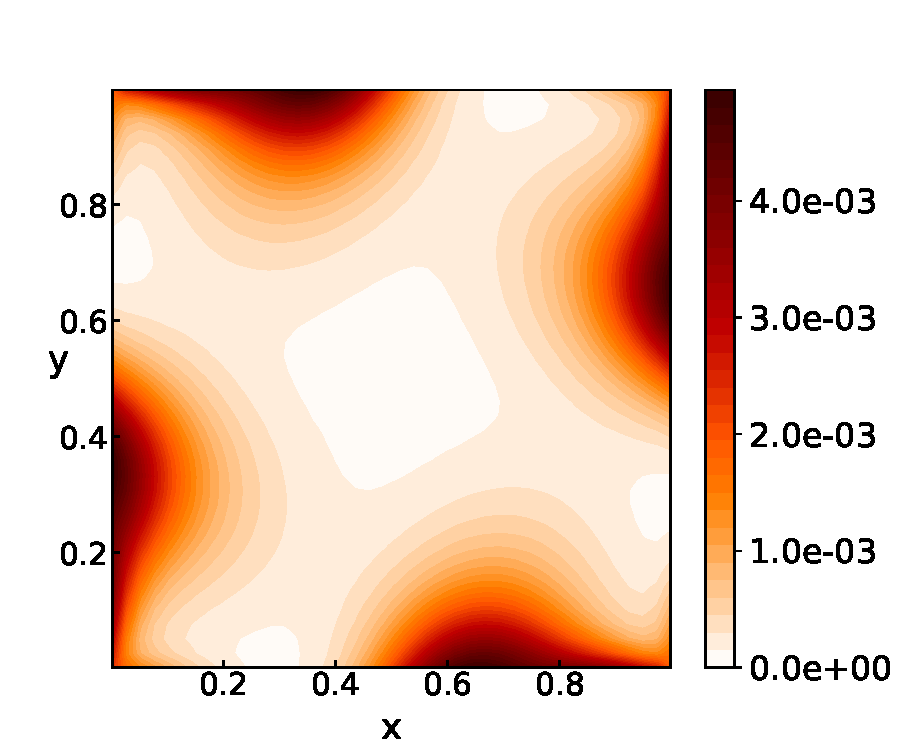
\includegraphics[width=\textwidth]{figures/delta_sigma_a3-sigma_t6-g0_5-r5-v9-phi_label.pdf}
        \caption{$\ANN (I_{-}^{(1)} + I_{-}^{(2)})$ 对应的密度 $\Phi$}
    \end{subfigure}
    \hfill
    \begin{subfigure}[b]{0.30\textwidth}
        \centering
        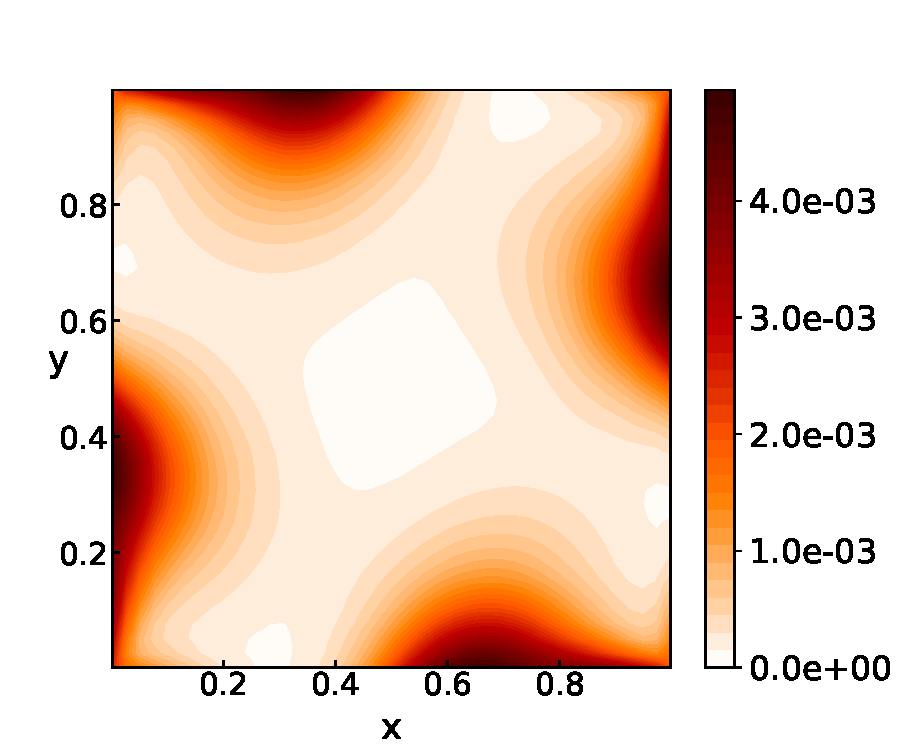
\includegraphics[width=\textwidth]{figures/delta_sigma_a3-sigma_t6-g0_5-r5-v9-phi_pre.pdf}
        \caption{$\ANN I_{-}^{(1)} + \ANN I_{-}^{(2)}$ 对应的密度 $\Phi$}
    \end{subfigure}
    \hfill
    \begin{subfigure}[b]{0.30\textwidth}
        \centering
        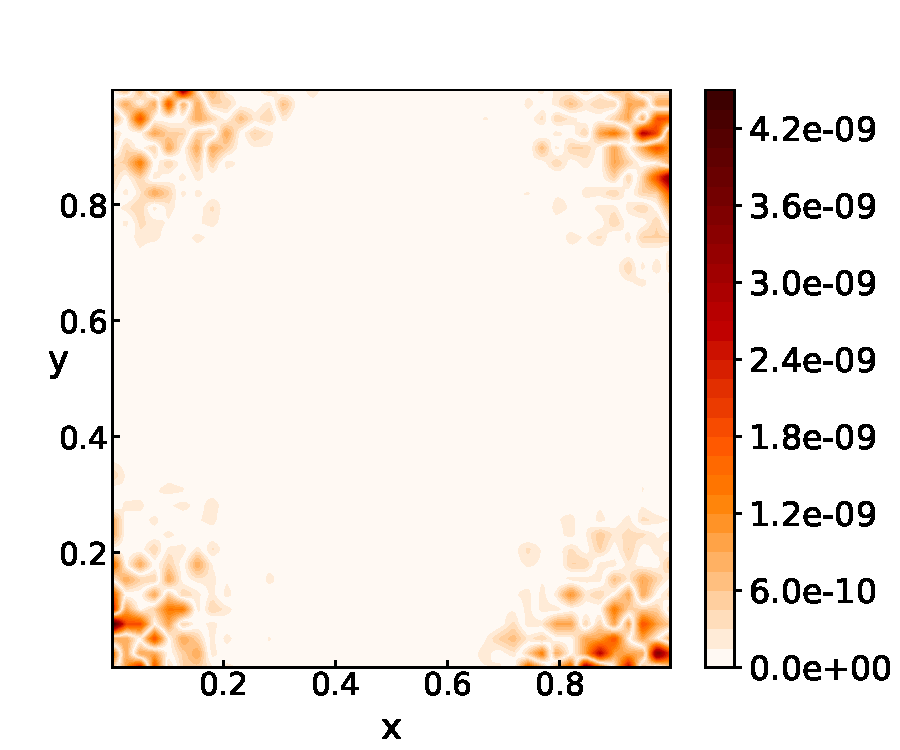
\includegraphics[width=\textwidth]{figures/delta_sigma_a3-sigma_t6-g0_5-r5-v9-phi_error.pdf}
        \caption{绝对误差}
    \end{subfigure}
    \bicaption{DeepRTE 可加性检验算例，参数取 $g=0.5$、$\mus=3$、$\mut=6$。}{Additivity verification of DeepRTE with $g=0.5$, $\mus=3$ and $\mut=6$.}
    \label{fig:additivity}
\end{figure}

\paragraph{2. 齐次性检验}
线性齐次性要求：若将入射边界整体按系数 $\alpha$ 放缩，则预测解也按同一系数放缩：
\begin{equation}\label{eq:homogeneity-val}
    \ANN(\alpha I_{-}) = \alpha \,\ANN I_{-}, \quad \forall\, \alpha \in \mathbb{R}.
\end{equation}
我们同样从验证集中选取边界条件 $I_{-}$：
\begin{equation}
    I_{-}:
    \begin{cases}
        y_l'=0.3875,\; y_r'=0.6125,\; x_b'=0.6125,\; x_t'=0.3875,   \\
        c_l'=0.6931,\; c_r'=-0.6931,\; c_b'=0.2871,\; c_t'=-0.2871, \\
        s_l'=-0.2871,\; s_r'=0.2871,\; s_b'=0.6931,\; s_t'=-0.6931,
    \end{cases}
\end{equation}
方差取 $\sigma_{\br}=0.01$、$\sigma_{\bOmega}=0.0075$，并令
\begin{equation}
    \alpha = 5.
\end{equation}
计算~\eqref{eq:homogeneity-val} 左右两侧的 MSE：
\begin{equation}
    \ell(\ANN (\alpha I_{-}), \alpha \,\ANN I_{-}) = 5.179\times 10^{-13},
\end{equation}
同样表明 DeepRTE 在数值上严格满足齐次性性质。

在此基础上，对于放缩边界 $\alpha I_{-}$，我们比较 DeepRTE 预测解 $\ANN (\alpha I_{-})$ 与数值求解器给出的真解 $\mathcal{A}(\alpha I_{-})$：MSE 为 $5.842\times10^{-9}$，RMSPE 为 $2.19\%$，说明在幅值放大的情形下模型依然保持较高精度。对应密度 $\Phi$ 的可视化结果如图~\ref{fig:homogeneity} 所示。

\begin{figure}[!htp]
    \centering
    \begin{subfigure}[b]{0.30\textwidth}
        \centering
        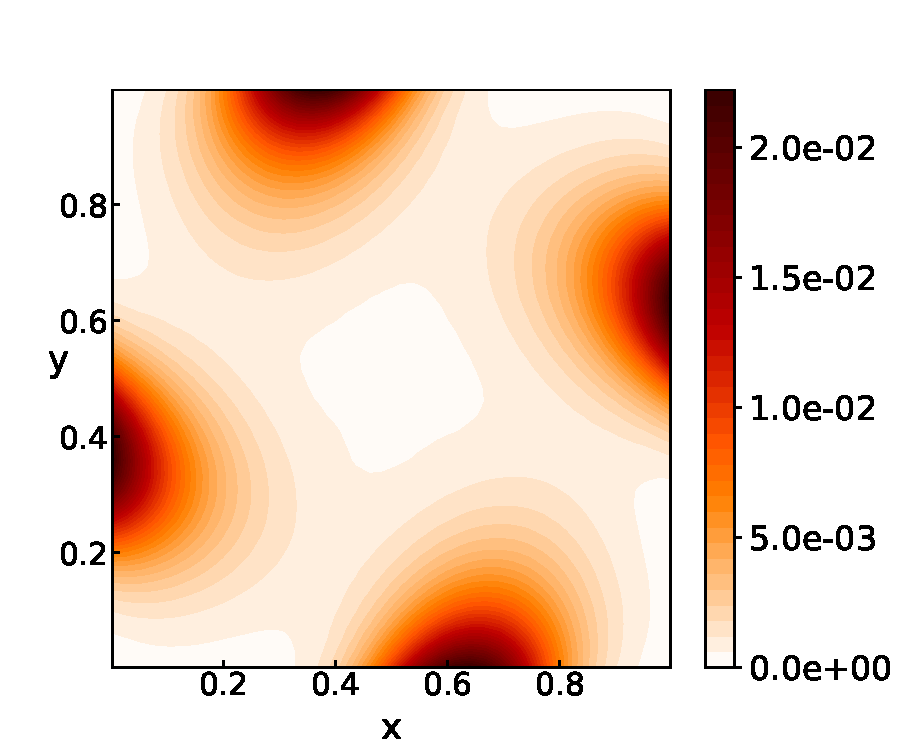
\includegraphics[width=\textwidth]{figures/delta-sigma_a3_sigma_t6-g0_5-r15-v3-phi_label.pdf}
        \caption{$\ANN (\alpha I_{-})$ 对应的密度 $\Phi$}
    \end{subfigure}
    \hfill
    \begin{subfigure}[b]{0.30\textwidth}
        \centering
        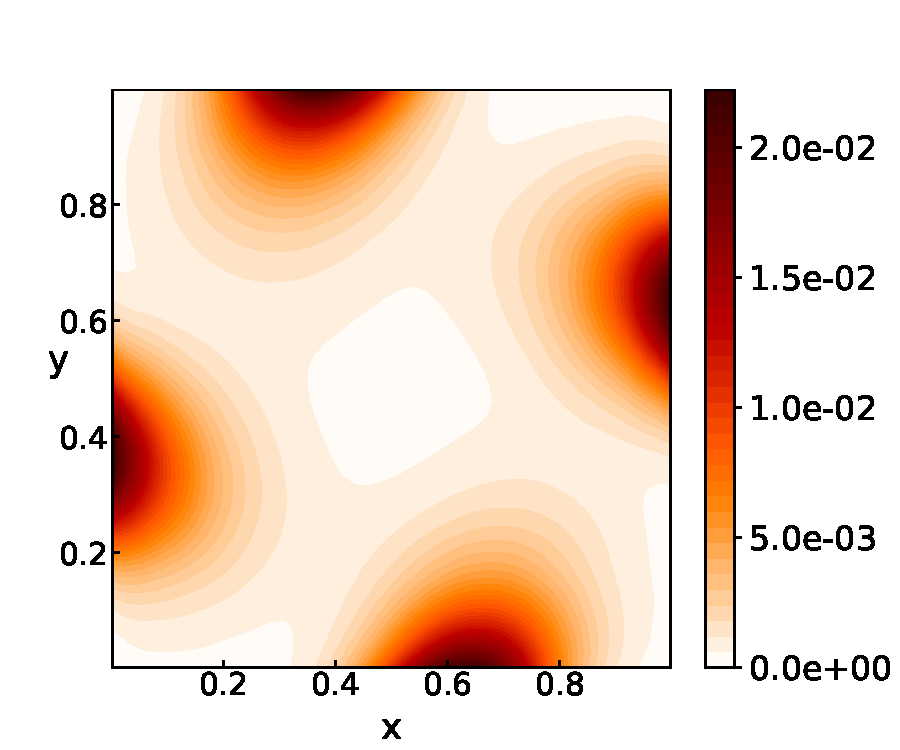
\includegraphics[width=\textwidth]{figures/delta-sigma_a3_sigma_t6-g0_5-r15-v3-phi_pre.pdf}
        \caption{$\alpha \,\ANN I_{-}$ 对应的密度 $\Phi$}
    \end{subfigure}
    \hfill
    \begin{subfigure}[b]{0.30\textwidth}
        \centering
        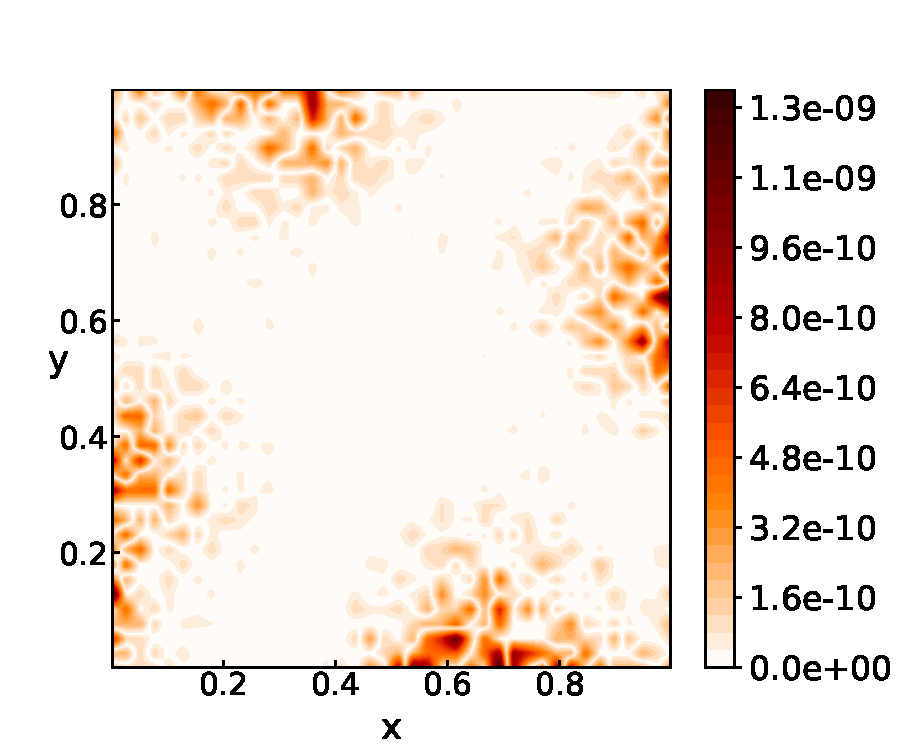
\includegraphics[width=\textwidth]{figures/delta-sigma_a3_sigma_t6-g0_5-r15-v3-phi_error.pdf}
        \caption{绝对误差}
    \end{subfigure}
    \bicaption{DeepRTE 齐次性检验算例，参数取 $g=0.5$、$\mus=3$、$\mut=6$、$\alpha=5$。}{Homogeneity verification with $g=0.5$, $\mus=3$, $\mut=6$ and $\alpha=5$.}\label{fig:homogeneity}
\end{figure}

同样地，我们在 100 个验证样本上统计检验齐次性。令缩放因子 $\alpha \sim \mathcal{U}(0,5)$，对每个原始边界条件 $I_{-}$ 构造 $\alpha I_{-}$，比较~\eqref{eq:homogeneity-val} 两侧。此时 MSE 与 RMSPE 分别为 $2.804\times 10^{-13}$ 与 $1.01\times 10^{-5}\%$，结果见表~\ref{tab:linearity}。

\begin{table}[!htp]
    \centering
    \begin{tabular}{lcc}
        \toprule
                         & MSE                    & RMSPE($\%$)          \\
        \midrule
        可加性（Additivity）  & $1.421\times 10^{-19}$ & $9.20\times 10^{-6}$ \\
        齐次性（Homogeneity） & $2.804\times 10^{-13}$ & $1.01\times 10^{-5}$ \\
        \bottomrule
    \end{tabular}
    \bicaption{在 $g=0.5$、与训练集分布一致的验证数据上对可加性与齐次性进行统计检验的结果。}{Additivity and homogeneity verification on 100 validation samples with the same distribution as the training dataset at $g=0.5$ (see Sec.~\ref{sec:acc}).}\label{tab:linearity}
\end{table}

\paragraph{3. 线性组合与误差分解}
前述可加性与齐次性表明：对于任意入射边界 $I_{-}$，DeepRTE 的泛化误差可以如定理~\ref{thm:error-estimate} 所示进行分解。本小节通过一个平滑入射边界算例，对该误差分解进行经验验证，并评估各个误差分量的相对量级。

考虑只在左边界施加平滑入射、其余边界为零的情形：
\begin{equation}
    \left \{ % tex-fmt: skip
    \begin{aligned}
         & I_-(x=0,y,c>0,s) = \sin(\pi y), \\
         & I_-(x=1,y,c<0,s) = 0,           \\
         & I_-(x,y=0,c,s>0) = 0,           \\
         & I_-(x,y=1,c,s<0) = 0.
    \end{aligned}
    \right. % tex-fmt: skip
\end{equation}

按照~\eqref{eq:particle-approx} 与~\eqref{eq:delta_defination}，仅需对左边界进行粒子近似：
\begin{equation}
    I_-(x=0,y,c>0,s) = \sin(\pi y) \approx \sum_{i=0}^{39} w_{i} \,\delta^{\sigma_{\br}}_{\{y_i\}}(y),
\end{equation}
其中 $\{y_i\}$ 为均匀网格中心，$g=0.5$、$\sigma_{\br} = 0.01$，并根据~\cite{chertock2017practical} 第 2.1 节取
\begin{equation}
    w_i=\frac{1}{40}\sin(\pi y_i).
\end{equation}

以数值解为参考解 $I^{\text{ref}}$，我们依次计算以下误差（所有 $L^2$ 误差均采用离散网格上的求积近似）：首先是正则化 Delta 近似误差
\begin{equation}
    \|I_{-} - I^{40}_{-,0.01}\|_{L^2} \approx \frac{1}{160}\bigl\|I_{(x=0,y,c>0,s)} - \sum_{i=0}^{39} w_{i} \,\delta^{\sigma_{\br}}_{\{y_i\}}(y)\bigr\|_{\ell^2}=4.799\times 10^{-5},
\end{equation}
以及
\begin{equation}
    \|\ANN_{\theta^*}(I_{-} - I^{40}_{-,0.01})\|_{L^2}\approx 2.190\times 10^{-7}, \quad
    \|\mathcal{A}(I_{-} - I^{40}_{-,0.01})\|_{L^2} \approx 2.208\times 10^{-7},
\end{equation}
最后是关于粒子近似的泛化误差项
\begin{equation}
    \| (\ANN_{\theta^*} - \mathcal{A}) I^{40}_{-,0.01}\|_{L^2}
    =\Bigl\|\sum_{i=0}^{39}w_i(\ANN_{\theta^*} - \mathcal{A}) \,\delta^{\sigma_{\br}}_{\{y_i\}}(y)\Bigr\|_{L^2} \leq \sum_{i=0}^{39}|w_i|\,\|(\ANN_{\theta^*} - \mathcal{A}) \,\delta^{\sigma_{\br}}_{\{y_i\}}(y)\|_{L^2} \approx 8.385\times 10^{-5}.
\end{equation}
由此得到总误差上界约为 $8.385\times 10^{-5}$。直接计算原边界条件下的推理误差
\begin{equation}
    \|(\ANN_{\theta^*} - \mathcal{A}) I_{-}\|_{L^2} \approx 1.888\times 10^{-5},
\end{equation}
明显低于上述理论上界，从数值上支持了定理~\ref{thm:error-estimate} 的误差分解结论。

\subsubsection{迁移学习与零样本性能}

本小节考察 DeepRTE 框架在迁移学习与零样本（Zero-Shot）场景下的表现。迁移学习允许模型将某一任务上学到的知识迁移到相关任务，以提升后者的性能；零样本能力则指在不额外训练的情况下，将模型直接应用于全新的条件。为展示 DeepRTE 在 RTE 问题上的此类能力——特别是其在几乎不做额外训练的前提下，适应新边界条件的能力——我们首先在 Delta 函数型入射边界条件数据集上训练模型，以学习 RTE 的基本物理规律；随后，在与训练集分布完全不同的边界条件上对模型进行测试，评估其泛化与零样本外推性能。

具体而言，我们考虑以下三类典型边界条件：
\begin{itemize}
    \item \textbf{Case I（常值边界条件）}: 从 Delta 函数边界条件外推到常值源项，用于评估模型的基础泛化能力；
    \item \textbf{Case II（三角函数边界条件）}: 通过正弦函数在空间方向上引入变化，用于检验模型处理平滑、周期且空间相关边界条件的能力；
    \item \textbf{Case III（速度相关边界条件）}: 在空间与速度方向上同时引入非线性依赖，用于评估模型对复杂、方向相关边界条件的适应能力。
\end{itemize}

\paragraph{Case I. 常值边界条件}
该算例的入射边界条件为
\begin{equation}
    \left \{
    \begin{aligned}
         & I_-(x=0,y,c>0,s) =1,  \\
         & I_-(x=1,y,c<0,s) = 0, \\
         & I_-(x,y=0,c,s>0) =0,  \\
         & I_-(x,y=1,c,s<0) =0,
    \end{aligned}
    \right.
\end{equation}

\begin{figure}[!htp]
    \centering
    \begin{subfigure}[b]{0.24\textwidth}
        \centering
        
\includegraphics[width=\textwidth]{test_bc1_g0.1_label_3d.pdf}
        \caption{$\Phi_{\text{label}}$ (3D)}\label{fig:caseI_label_3d}
    \end{subfigure}
    \hfill
    \begin{subfigure}[b]{0.24\textwidth}
        \centering
        
\includegraphics[width=\textwidth]{test_bc1_g0.1_label.pdf}
        \caption{$\Phi_{\text{label}}$}\label{fig:caseI_label}
    \end{subfigure}
    \hfill
    \begin{subfigure}[b]{0.24\textwidth}
        \centering
        
\includegraphics[width=\textwidth]{test_bc1_g0.1_pre.pdf}
        \caption{$\Phi_{\text{predict}}$}\label{fig:caseI_predict}
    \end{subfigure}
    \hfill
    \begin{subfigure}[b]{0.24\textwidth}
        \centering
        
\includegraphics[width=\textwidth]{test_bc1_g0.1_error.pdf}
        \caption{Absolute error}\label{fig:caseI_error}
    \end{subfigure}
    \bicaption{常值边界条件（Case I）下的评估结果，散射核参数 $g\in (0,0.2)$。预测解的 RMSPE 为 2.573\%。}{Evaluation dataset with scattering kernel coefficient $g\in (0,0.2)$. The RMSPE of the predicted solution is 2.573\%.}
\end{figure}

\paragraph{Case II. 三角函数边界条件}
该算例的边界条件为
\begin{equation}
    \left \{
    \begin{aligned}
         & I_-(x=0,y,c>0,s) =a_L\sin{k_L y}+5,   \\
         & I_-(x=1,y,c<0, s) = a_R\sin{k_R y}+5, \\
         & I_-(x,y=0,c,s>0) =a_B\sin{k_B x}+5,   \\
         & I_-(x,y=1,c,s<0) =a_T\sin{k_T x}+5,
    \end{aligned}
    \right.
\end{equation}
其中
\begin{equation}
    a_L, a_R, a_B, a_T \sim \mathcal{U}(-5,5), \quad
    k_L, k_R, k_B, k_T \sim\mathcal{U}(-10, 10).
\end{equation}

\begin{figure}[!htp]
    \centering
    \begin{subfigure}[b]{0.24\textwidth}
        \centering
        
\includegraphics[width=\textwidth]{test_sin_g0.1_label_3d.pdf}
        \caption{$\Phi_{\text{label}}$ (3D)}\label{fig:caseII_label_3d}
    \end{subfigure}
    \hfill
    \begin{subfigure}[b]{0.24\textwidth}
        \centering
        
\includegraphics[width=\textwidth]{test_sin_g0.1_label.pdf}
        \caption{$\Phi_{\text{label}}$}\label{fig:caseII_label}
    \end{subfigure}
    \hfill
    \begin{subfigure}[b]{0.24\textwidth}
        \centering
        
\includegraphics[width=\textwidth]{test_sin_g0.1_pre.pdf}
        \caption{$\Phi_{\text{predict}}$}\label{fig:caseII_predict}
    \end{subfigure}
    \hfill
    \begin{subfigure}[b]{0.24\textwidth}
        \centering
        
\includegraphics[width=\textwidth]{test_sin_g0.1_error.pdf}
        \caption{Absolute error}\label{fig:caseII_error}
    \end{subfigure}
    \bicaption{三角函数边界条件（Case II）下的评估结果，散射核参数 $g\in (0,0.2)$。预测解的 RMSPE 为 1.968\%。}{Evaluation data set with scattering kernel coefficient $g\in (0,0.2)$. The RMSPE of the predict solution is 1.968\%.}
\end{figure}

\paragraph{Case III. 速度相关边界条件}
该算例的边界条件为
\begin{equation}
    \left \{
    \begin{aligned}
         & I_-(x=0,y,c>0,s) =(a_{Lr}\sin{k_{Lr} y}+5)(a_{Lv}\sin{k_{Lv} c}+1)(a_{Lv}\sin{k_{Lv} s}+1),  \\
         & I_-(x=1,y,c<0,s) = (a_{Rr}\sin{k_{Rr} y}+5)(a_{Rv}\sin{k_{Rv} c}+1)(a_{Rv}\sin{k_{Rv} s}+1),
        \\
         & I_-(x,y=0,c,s>0) =(a_{Br}\sin{k_{Br} x}+5)(a_{Bv}\sin{k_{Bv} c}+1)(a_{Bv}\sin{k_{Bv} s}+1),
        \\
         & I_-(x,y=1,c,s<0) =(a_{Tr}\sin{k_{Tr} x}+5)(a_{Tv}\sin{k_{Tv} c}+1)(a_{Tv}\sin{k_{Tv} s}+1),
    \end{aligned}
    \right.
\end{equation}
其中
\begin{equation}
    \begin{aligned}
        a_{Lr}, a_{Rr}, a_{Br}, a_{Tr} & \sim \mathcal{U}(-5,5),   \\
        a_{Lv}, a_{Rv}, a_{Bv}, a_{Tv} & \sim \mathcal{U}(-1,1),   \\
        k_{Lr}, k_{Rr}, k_{Br}, k_{Tr} & \sim\mathcal{U}(-10, 10), \\
        k_{Lv}, k_{Rv}, k_{Bv}, k_{Tv} & \sim\mathcal{U}(-6, 6).
    \end{aligned}
\end{equation}

\begin{figure}[!htp]
    \centering
    \begin{subfigure}[b]{0.24\textwidth}
        \centering
        
\includegraphics[width=\textwidth]{test_sin_rv_g0.1_label_3d.pdf}
        \caption{$\Phi_{\text{label}}$ (3D)}\label{fig:caseIII_label_3d}
    \end{subfigure}
    \hfill
    \begin{subfigure}[b]{0.24\textwidth}
        \centering
        
\includegraphics[width=\textwidth]{test_sin_rv_g0.1_label.pdf}
        \caption{$\Phi_{\text{label}}$}\label{fig:caseIII_label}
    \end{subfigure}
    \hfill
    \begin{subfigure}[b]{0.24\textwidth}
        \centering
        
\includegraphics[width=\textwidth]{test_sin_rv_g0.1_pre.pdf}
        \caption{$\Phi_{\text{predict}}$}\label{fig:caseIII_predict}
    \end{subfigure}
    \hfill
    \begin{subfigure}[b]{0.24\textwidth}
        \centering
        
\includegraphics[width=\textwidth]{test_sin_rv_g0.1_error.pdf}
        \caption{Absolute error}\label{fig:caseIII_error}
    \end{subfigure}
    \bicaption{速度相关边界条件（Case III）下的评估结果，散射核参数 $g\in (0,0.2)$。预测解的 RMSPE 为 1.908\%。}{Evaluation data set with scattering kernel coefficient $g\in (0,0.2)$. The RMSPE of the predict solution is 1.908\%.}
\end{figure}

\begin{table}[!htp]
    \centering
    \begin{tabular}{@{}cccc@{}}
        \toprule
                                  & 测试数据集           & MSE                    & RMSPE (\%) \\ \midrule
        \multirow{3}{*}{Case I}   & $g\in(0,0.2)$   & $4.390 \times 10^{-6}$ & 1.833      \\
                                  & $g\in(0.4,0.6)$ & $5.184 \times 10^{-6}$ & 1.994      \\
                                  & $g\in(0.7,0.9)$ & $1.474 \times 10^{-5}$ & 3.193      \\ \midrule
        \multirow{3}{*}{Case II}  & $g\in(0,0.2)$   & $4.931 \times 10^{-4}$ & 1.653      \\
                                  & $g\in(0.4,0.6)$ & $5.798 \times 10^{-4}$ & 1.827      \\
                                  & $g\in(0.7,0.9)$ & $2.870 \times 10^{-3}$ & 3.572      \\ \midrule
        \multirow{3}{*}{Case III} & $g\in(0,0.2)$   & $1.065 \times 10^{-3}$ & 2.383      \\
                                  & $g\in(0.4,0.6)$ & $1.127 \times 10^{-3}$ & 2.452      \\
                                  & $g\in(0.7,0.9)$ & $1.853 \times 10^{-3}$ & 3.069      \\ \bottomrule
    \end{tabular}
    \bicaption{迁移学习与零样本实验结果。模型在 Delta 函数边界条件上训练后，分别在常值边界（Case I）、三角函数边界（Case II）与空间–速度复合三角边界（Case III）上测试，给出了不同 $g$ 区间下的 MSE 与 RMSPE。}{Transfer learning and Zero-Shot performance. The model, trained on delta function boundary conditions, is tested on constant (Case I), trigonometric (Case II), and combined trigonometric (Case III) boundary conditions for $g$ in ranges (0,0.2), (0.4,0.6), and (0.7,0.9). Performance is measured using mean squared error (MSE) and root mean square percentage error (RMSPE), demonstrating robust generalization with errors below 3.2\% for Case I, 3.6\% for Case II, and 3.1\% for Case III.}
\end{table}

\paragraph{高度前向散射下的分布外泛化（$g=0.99$）}

最后，我们考察 DeepRTE 在散射核超出预训练数据集分布时的表现。具体而言，我们令散射不对称参数 $g$ 逼近 1，并在 $g=0.99$ 的高度前向散射情形下进行测试。实验设置为
\begin{equation}
    \mu_t(x,y) =
    \begin{cases}
        6,  & \text{若 } (x,y) \in D_\mu,    \\
        10, & \text{若 } (x,y) \notin D_\mu,
    \end{cases}
    \quad
    \mu_s(x,y) =
    \begin{cases}
        3, & \text{若 } (x,y) \in D_\mu,    \\
        5, & \text{若 } (x,y) \notin D_\mu,
    \end{cases}
    \quad D_\mu = [0.4, 0.6]^2,
\end{equation}
入射边界条件取为
\begin{equation}
    \left \{ % tex-fmt: skip
    \begin{aligned}
         & I_-(x=0,y,c>0,s) =(5\sin{2\pi y}+5)(\sin{\pi c}+1)(\sin{\pi s}+1),  \\
         & I_-(x=1,y,c<0,s) = (5\sin{2\pi y}+5)(\sin{\pi c}+1)(\sin{\pi s}+1), \\
         & I_-(x,y=0,c,s>0) =(5\sin{2\pi x}+5)(\sin{\pi c}+1)(\sin{\pi s}+1),  \\
         & I_-(x,y=1,c,s<0) =(5\sin{2\pi x}+5)(\sin{\pi c}+1)(\sin{\pi s}+1).
    \end{aligned}
    \right. % tex-fmt: skip
\end{equation}

\begin{figure}[!htp]
    \centering
    \begin{subfigure}[t]{0.32\textwidth}
        \centering
        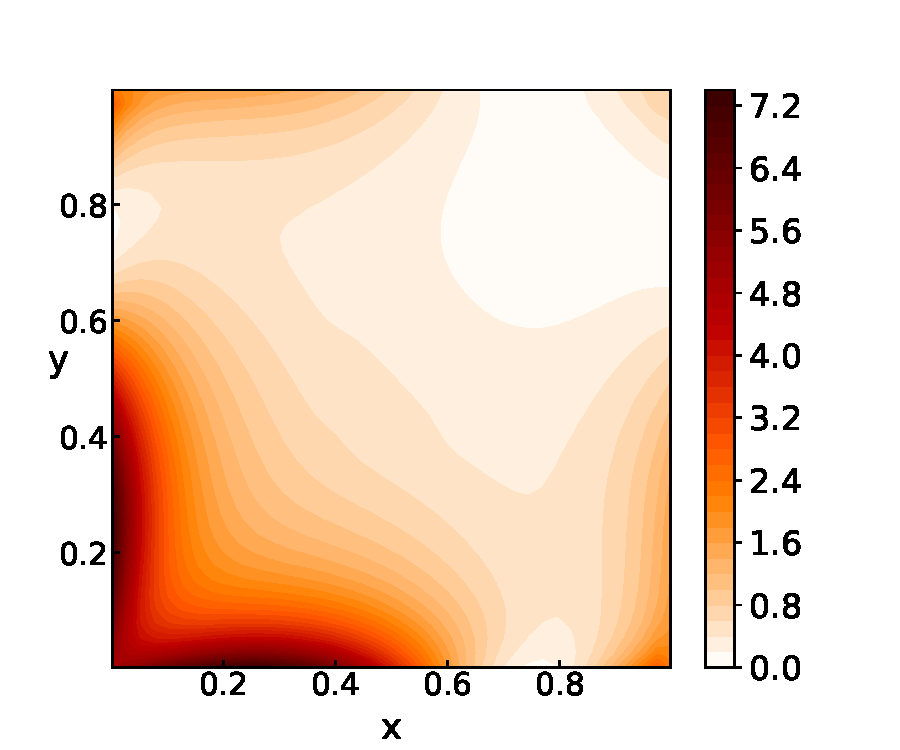
\includegraphics[width=\linewidth]{figures/test_g0.99_phi_label.pdf}
        \caption{$\Phi_{\text{label}}$}
        \label{fig:deeprte-g099-label}
    \end{subfigure}\hfill
    \begin{subfigure}[t]{0.32\textwidth}
        \centering
        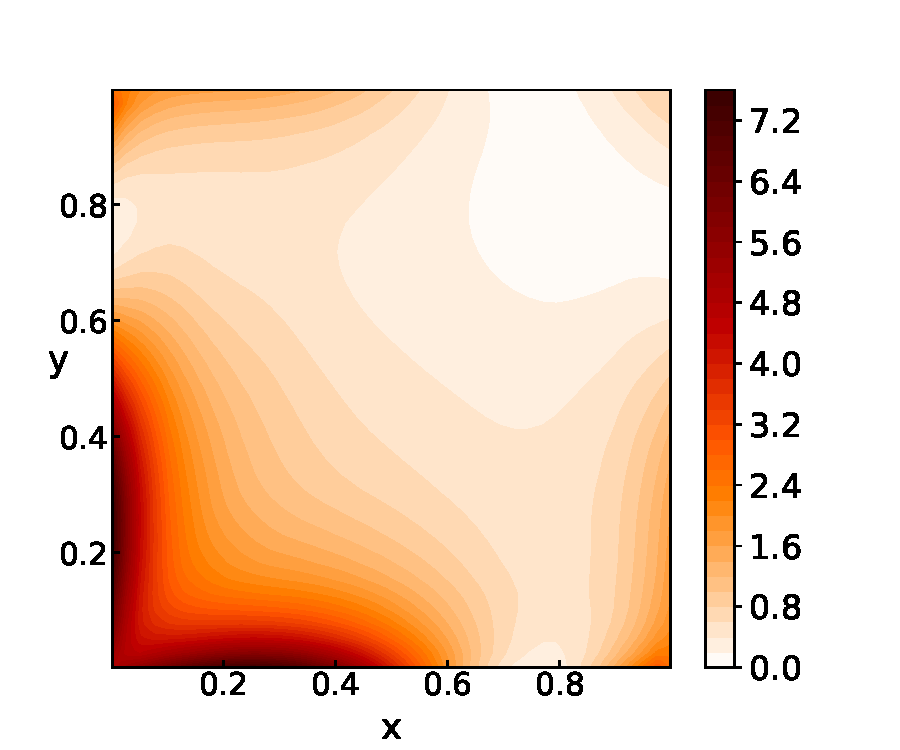
\includegraphics[width=\linewidth]{figures/test_g0.99_phi_pre.pdf}
        \caption{$\Phi_{\text{predict}}$}
        \label{fig:deeprte-g099-predict}
    \end{subfigure}\hfill
    \begin{subfigure}[t]{0.32\textwidth}
        \centering
        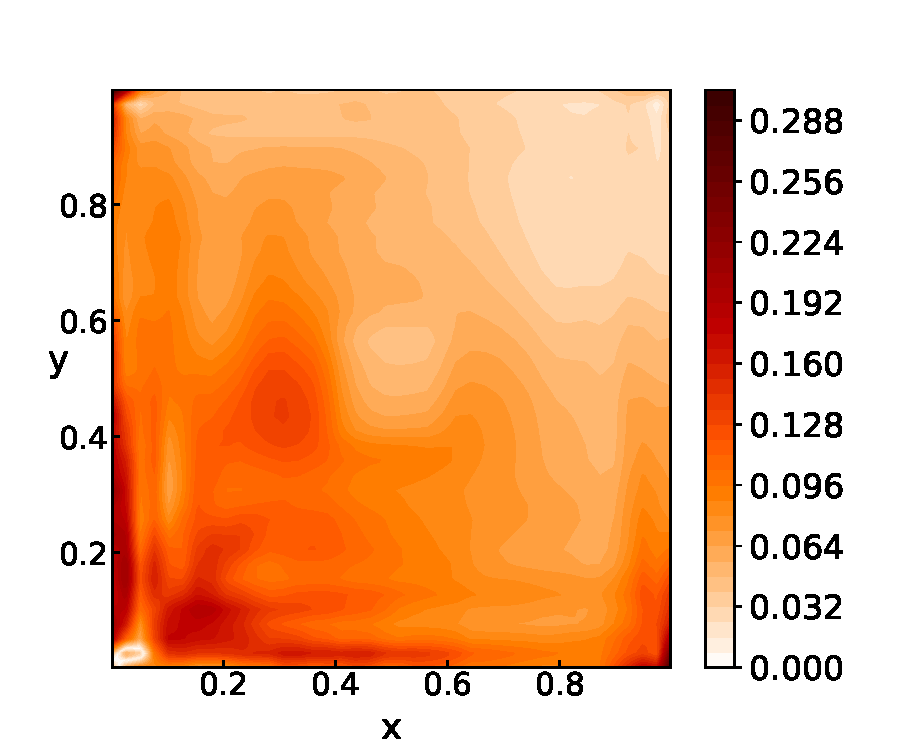
\includegraphics[width=\linewidth]{figures/test_g0.99_phi_error.pdf}
        \caption{Absolute error}
        \label{fig:deeprte-g099-error}
    \end{subfigure}
    \bicaption{在 $g=0.99$ 高度前向散射情形下 DeepRTE 的预测结果与真值比较。}{DeepRTE evaluation at $g=0.99$.}
    \label{fig:deeprte-g099}
\end{figure}

图~\ref{fig:deeprte-g099} 展示了参考解密度 $\Phi_{\text{label}}$、预测解密度 $\Phi_{\text{predict}}$ 及其绝对误差。即便在 $g$ 极接近 1、散射高度各向异性的极端情形下，DeepRTE 仍保持了较高预测精度：该算例下 MSE 为 $7.64\times 10^{-3}$，RMSPE 为 $4.257\%$。这表明 DeepRTE 在接近奇异的强前向散射区间仍具有良好的稳健性和分布外泛化能力，能够有效求解高度前向集中的辐射传输问题。

综上，DeepRTE 在迁移学习与零样本场景下均展现出较强的表达能力与外推能力。依托在 Delta 函数边界条件上学到的核心物理结构，模型即便在完全不同的边界条件下、甚至在未见过的场景中，也能给出精度较高的预测结果。这表明基于深度学习的算子框架在科学计算领域具有广阔的应用前景。

\subsection{网格依赖性与跨分辨率性能}

数值方法在不同网格分辨率下的表现是评价其实用性的重要指标之一。本小节考察 DeepRTE 的“网格独立性”性质：即在细网格上训练得到的参数能否在较粗网格上仍然保持较高精度。

\begin{table}[!htp]
    \centering
    \begin{tabular}{cccc}
        \toprule
        测试数据集 & 网格分辨率         & MSE                    & RMSPE (\%) \\
        \midrule
        \multirow{3}{*}{Evaluation Dataset}
              & $40\times 40$ & $5.453\times 10^{-10}$ &
        $2.759$                                                     \\
              & $20\times 20$ & $8.235 \times 10^{-9}$ &
        $10.006$                                                    \\
              & $10\times 10$ & $9.476 \times 10^{-8}$ &
        $34.346$                                                    \\
        \midrule
        \multirow{3}{*}{Case I}
              & $40\times 40$ & $4.390 \times 10^{-6}$ &
        $1.833$                                                     \\
              & $20\times 20$ & $1.876 \times 10^{-5}$ &
        $3.758$                                                     \\
              & $10\times 10$ & $1.243 \times 10^{-4}$ &
        $9.276$                                                     \\
        \midrule
        \multirow{3}{*}{Case II}
              & $40\times 40$ & $4.931 \times 10^{-4}$ &
        $1.653$                                                     \\
              & $20\times 20$ & $1.792 \times 10^{-2}$ &
        $9.952$                                                     \\
              & $10\times 10$ & $3.687 \times 10^{-2}$ &
        $13.798$                                                    \\
        \midrule
        \multirow{3}{*}{Case III}
              & $40\times 40$ & $1.065 \times 10^{-3}$ &
        $2.383$                                                     \\
              & $20\times 20$ & $1.175 \times 10^{-2}$ &
        $8.132$                                                     \\
              & $10\times 10$ & $4.511 \times 10^{-2}$ &
        $15.477$                                                    \\
        \bottomrule
    \end{tabular}
    \bicaption{DeepRTE 在不同网格分辨率与测试集上的表现。评价数据集在 $40\times 40$ 网格上可达到 $5.45\times10^{-10}$ 的 MSE，而在粗网格上误差随分辨率下降而单调增大；Case I--III 亦表现出类似趋势。}{Performance of DeepRTE across different resolutions and test sets. The Evaluation Dataset shows very high precision, with an MSE of $5.45\times10^{-10}$ on the $40\times 40$ grid. In contrast, Cases I-III show a consistent increase in error on coarser grids. This increase is mainly because of the limitations of numerical integration. With the second-order midpoint rule, halving the grid resolution should theoretically make the integration error four times larger, which matches our findings.}\label{tab:mesh_independence_multiple_testsets}
\end{table}

从表~\ref{tab:mesh_independence_multiple_testsets} 可以看出：对于评价数据集与 Case I，RMSPE 在 $40\times 40$ 网格上的范围约为 $1.8$--$2.8\%$，当网格减半至 $20\times 20$ 时误差上升到约 $3.8$--$10\%$。Case II 与 Case III 的误差增幅略大，但仍处于可接受范围，在粗网格（$10\times 10$）上 RMSPE 约为 $8$--$15\%$。

这种误差随网格粗化而近似四倍增长的现象，与外层数值积分采用二阶中点公式的理论误差界一致：在二阶中点公式下，当网格尺寸减少一半时，积分误差理论上应放大约四倍。这一观察表明：在 Delta 函数边界条件问题中，DeepRTE 已经较好地学习到了基本解的结构，当前误差主要来源于数值积分本身，而非神经网络近似能力的瓶颈。因此，将来若采用更高阶的数值积分方法，有望在不显著增加网络复杂度的前提下进一步提升整体精度。

总体而言，DeepRTE 在不同网格分辨率下仍能保持较好的精度与稳定性，说明网络捕捉的是辐射传输方程的基本物理规律，而非简单地“记忆”某一固定网格上的解。这一网格独立性具有重要意义：
\begin{enumerate}
    \item 计算效率：用户可以在细网格上训练模型以获得高精度，然后在较粗网格上进行快速预测，在精度与效率之间灵活折中；
    \item 灵活性：同一组训练好的模型参数可以迁移到具有不同网格需求的问题中使用，而无需重新训练。
\end{enumerate}

